\documentclass[12pt, fullpage,letterpaper]{article}

\usepackage[margin=1in]{geometry}
\usepackage{url}
\usepackage{amsmath}
\usepackage{amssymb}
\usepackage{xspace}
\usepackage{graphicx}
\usepackage{hyperref}
\usepackage{listings}
\usepackage{graphicx}

\newcommand{\semester}{Spring 2020}
\newcommand{\assignmentId}{1}
\newcommand{\releaseDate}{21 January, 2020}

\newcommand{\bx}{{\bf x}}
\newcommand{\bw}{{\bf w}}

\title{CS 5350/6350: Machine Learining \semester}
\author{Homework \assignmentId \\* Britton Gaul \\* u0915408}

\begin{document}

\maketitle

\input{emacscomm}



\section{Decision Tree}

\begin{enumerate}
\item~ 
\begin{enumerate}
\item~
\newline $x_1: S_0 = 1, 2, 3, 5, 7; S_1 = 4, 6; (p_0^+, p_0^-)=(.2, .8); (p_1^+, p_1^-)=(.5, .5); H(S_0)=.72; H(S_1)=1; H(S)=.86;$  information gain = .06
\newline $x_2: S_0 = 1, 3, 4; S_1 = 2, 5, 6, 7; (p_0^+, p_0^-)=(2/3, 1/3); (p_1^+, p_1^-)=(0, 1); H(S_0)=.92; H(S_1)=0; H(S)=.86;$  information gain = .47
\newline $x_3: S_0 = 2, 4, 6, 7; S_1 = 1, 3, 5; (p_0^+, p_0^-)=(.25, .75); (p_1^+, p_1^-)=(1/3, 2/3); H(S_0)=.81; H(S_1)=.92; H(S)=.86;$  information gain = .03
\newline $x_4: S_0 = 1, 2, 5, 6; S_1 = 3, 4, 7; (p_0^+, p_0^-)=(0, 1); (p_1^+, p_1^-)=(2/3, 1/3); H(S_0)=0; H(S_1)=.92; H(S)=.86;$  information gain = .47
\newline The first split will be on $x_2$, because it has the highest information gain. As a result the subset to be further split is S = 1, 3, 4 where $x_2=0$
\newline $x_1: S_0 = 1, 3; S_1 = 4; (p_0^+, p_0^-)=(.5, .5); (p_1^+, p_1^-)=(1, 0); H(S_0)=1; H(S_1)=0; H(S)=.92;$  information gain = .25
\newline $x_3: S_0 = 4; S_1 = 1, 3; (p_0^+, p_0^-)=(1, 0); (p_1^+, p_1^-)=(.5, .5); H(S_0)=0; H(S_1)=1; H(S)=.92;$  information gain = .25
\newline $x_4: S_0 = 1; S_1 = 3, 4; (p_0^+, p_0^-)=(0, 1); (p_1^+, p_1^-)=(1, 0); H(S_0)=0; H(S_1)=0; H(S)=.92;$  information gain = .92
\newline The second split will be on $x_4$ because it was the largest infomration gain in the subset. For when $x_2=1$ the y value will always 0. 
\newline Tree:
\newline \includegraphics{cs5350hw1_1.jpg}
\item~
\newline Boolean function: $y=x_2' \wedge x_4$ 
\newline Table for function:
\begin{table}[h]
	\centering
	\begin{tabular}{cccc|c}
		$x_1$ & $x_2$ & $x_3$ & $x_4$ & $y$\\ 
		\hline\hline
		0 & 0 & 0 & 0 & 0 \\ \hline
		0 & 0 & 0 & 1 & 1 \\ \hline
		0 & 0 & 1 & 0 & 0 \\ \hline
		0 & 1 & 0 & 0 & 0 \\ \hline
		1 & 0 & 0 & 0.& 0\\ \hline
		0 & 0 & 1 & 1 & 1\\ \hline
		0 & 1 & 0 & 1 & 0\\ \hline
		0 & 1 & 1 & 0 & 0 \\ \hline
		1 & 0 & 0 & 1 & 1 \\ \hline
		1 & 0 & 1 & 0 & 0 \\ \hline
		1 & 1 & 0 & 0 & 0 \\ \hline
		0 & 1 & 1 & 1 & 0\\ \hline
		1 & 1 & 0 & 1 & 0\\ \hline
		1 & 0 & 1 & 1 & 1\\ \hline
		1 & 1 & 1 & 0 & 0\\ \hline
		1 & 1 & 1 & 1 & 0\\ \hline
	\end{tabular}
\end{table}

`\end{enumerate}
\item~ 
\begin{enumerate}
	\item~
	\newline First split:
	\newline -Outlook:
	\newline $S_s = 1, 2,8, 9, 11; p^+=2/5; Majority Error=.4$
	\newline $S_o=3, 7, 12, 13; p^+=4/4 = 1; Majority Error=0$
	\newline $S_r=4, 5, 6, 10, 14; p^+=3/5; Majority Error=.4$
	\newline $Information Gain=\frac{5}{14}-\frac{5}{14}\cdot (.4+.4)-\frac{4}{14} \cdot 0 = .07$
	\newline -Temperature:
	\newline $S_h = 1, 2, 3, 13; p^+=1/2; Majority Error=.5$
	\newline $S_m=4, 8, 10, 11, 12, 14; p^+=2/3; Majority Error=1/3$
	\newline $S_c=5, 6, 7, 9; p^+=3/4; Majority Error=.25$
	\newline $Information Gain=\frac{5}{14}-\frac{5}{14}\cdot (.5+.25)-\frac{6}{14} \cdot \frac{1}{3} = 0$
	\newline -Humidity:
	\newline $S_h = 1, 2, 3, 4, 8, 12, 14; p^+=3/7; Majority Error=3/7$
	\newline $S_n=5, 6, 7, 9, 10, 11, 13; p^+=6/7; Majority Error=1/7$
	\newline $S_l=none$
	\newline $Information Gain=\frac{5}{14}-\frac{7}{14}\cdot (\frac{3}{7}+\frac{1}{7}) = .07$
	\newline -Wind:
	\newline $S_s = 2, 6, 7, 11, 12, 14; p^+=1/2; Majority Error=.5$
	\newline $S_w=1, 3, 4, 5, 8, 9, 10, 13; p^+=3/4; Majority Error=.25$
	\newline $Information Gain=\frac{5}{14}-\frac{6}{14}\cdot (\frac{1}{2}-\frac{8}{14}) \cdot .25 = 0$
	\newline Outlook has the highest information gain so it will be used to split
	\newline
	\newline Second split of subsets:
	\newline Sunny subset 1, 2, 8, 9, 11:
	\newline -Temperature:
	\newline $S_h = 1, 2; p^+=0; Majority Error=0$
	\newline $S_m=8, 11, 14; p^+=1/2; Majority Error=.5$
	\newline $S_c=9; p^+=1; Majority Error=0$
	\newline $Information Gain=.4 \cdot \frac{2}{5} \cdot .5=.2$
	\newline -Humidity
	\newline $S_h = 1, 2, 8; p^+=0; Majority Error=0$
	\newline $S_n=9, 11; p^+=1; Majority Error=0$
	\newline $S_l=none$
	\newline $Information Gain=.4$
	\newline -Wind:
	\newline $S_s = 2,11; p^+=1/2; Majority Error=.5$
	\newline $S_w=1, 8, 9; p^+=1/3; Majority Error=\frac{1}{3}$
	\newline $Information Gain=.4-\frac{2}{5}\cdot.5-\frac{3}{5}\cdot\frac{1}{3} = 0$
	\newline Humidity has the largest information gain so it is used for the second split of the sunny subset of outlook
	\newline
	\newline The Humidity split has only two possible outcomes: 
	\newline $S_{sh}=1, 2, 8; p^+ =0$
	\newline $S_{sn}=9, 11; p^+ =1$
	\newline so this cannot be split anymore
	\newline
	\newline Overcast subset 3, 7, 12, 13:
	\newline For the overcast subset 3, 7, 12, 13; $p^+=1$ with Majority Error = 0, so this subset always results in 'yes'
	\newline
	\newline Rainy Subset 4, 5, 6, 10, 14:
	\newline -Temperature:
	\newline $S_h = none$
	\newline $S_m=4, 10, 14; p^+=2/3; Majority Error=.33$
	\newline $S_c=5, 6; p^+=1/2; Majority Error=.5$
	\newline $Information Gain=.4-\frac{3\cdot.33+2\cdot.5}{5}=0$
	\newline -Humidity
	\newline $S_h = 4, 14; p^+=1/2; Majority Error=.5$
	\newline $S_n=5, 6, 10; p^+=2/3; Majority Error=.33$
	\newline $S_l=none$
	\newline $Information Gain=.4-frac{2\cdot.5+3\cdot.33}{5}=0$
	\newline -Wind:
	\newline $S_s = 6, 14; p^+=0; Majority Error=0$
	\newline $S_w=4, 5, 10; p^+=1; Majority Error=0$
	\newline $Information Gain=.4$
	\newline Wind has the largest information gain from the rainy subset so it will be chosen to split. 
	\newline
	\newline The split subsets from the Rainy subset are:
	\newline $S_{rs}=6, 14; p^+=0; Majority Error = 0$
	\newline $S_{rw}=4, 5, 10; p^+=1; Majority Error = 0$
	\newline So the final result can be determined from this subset
	\newline
	\newline Final tree using Majority Error:
	\newline
	\newline 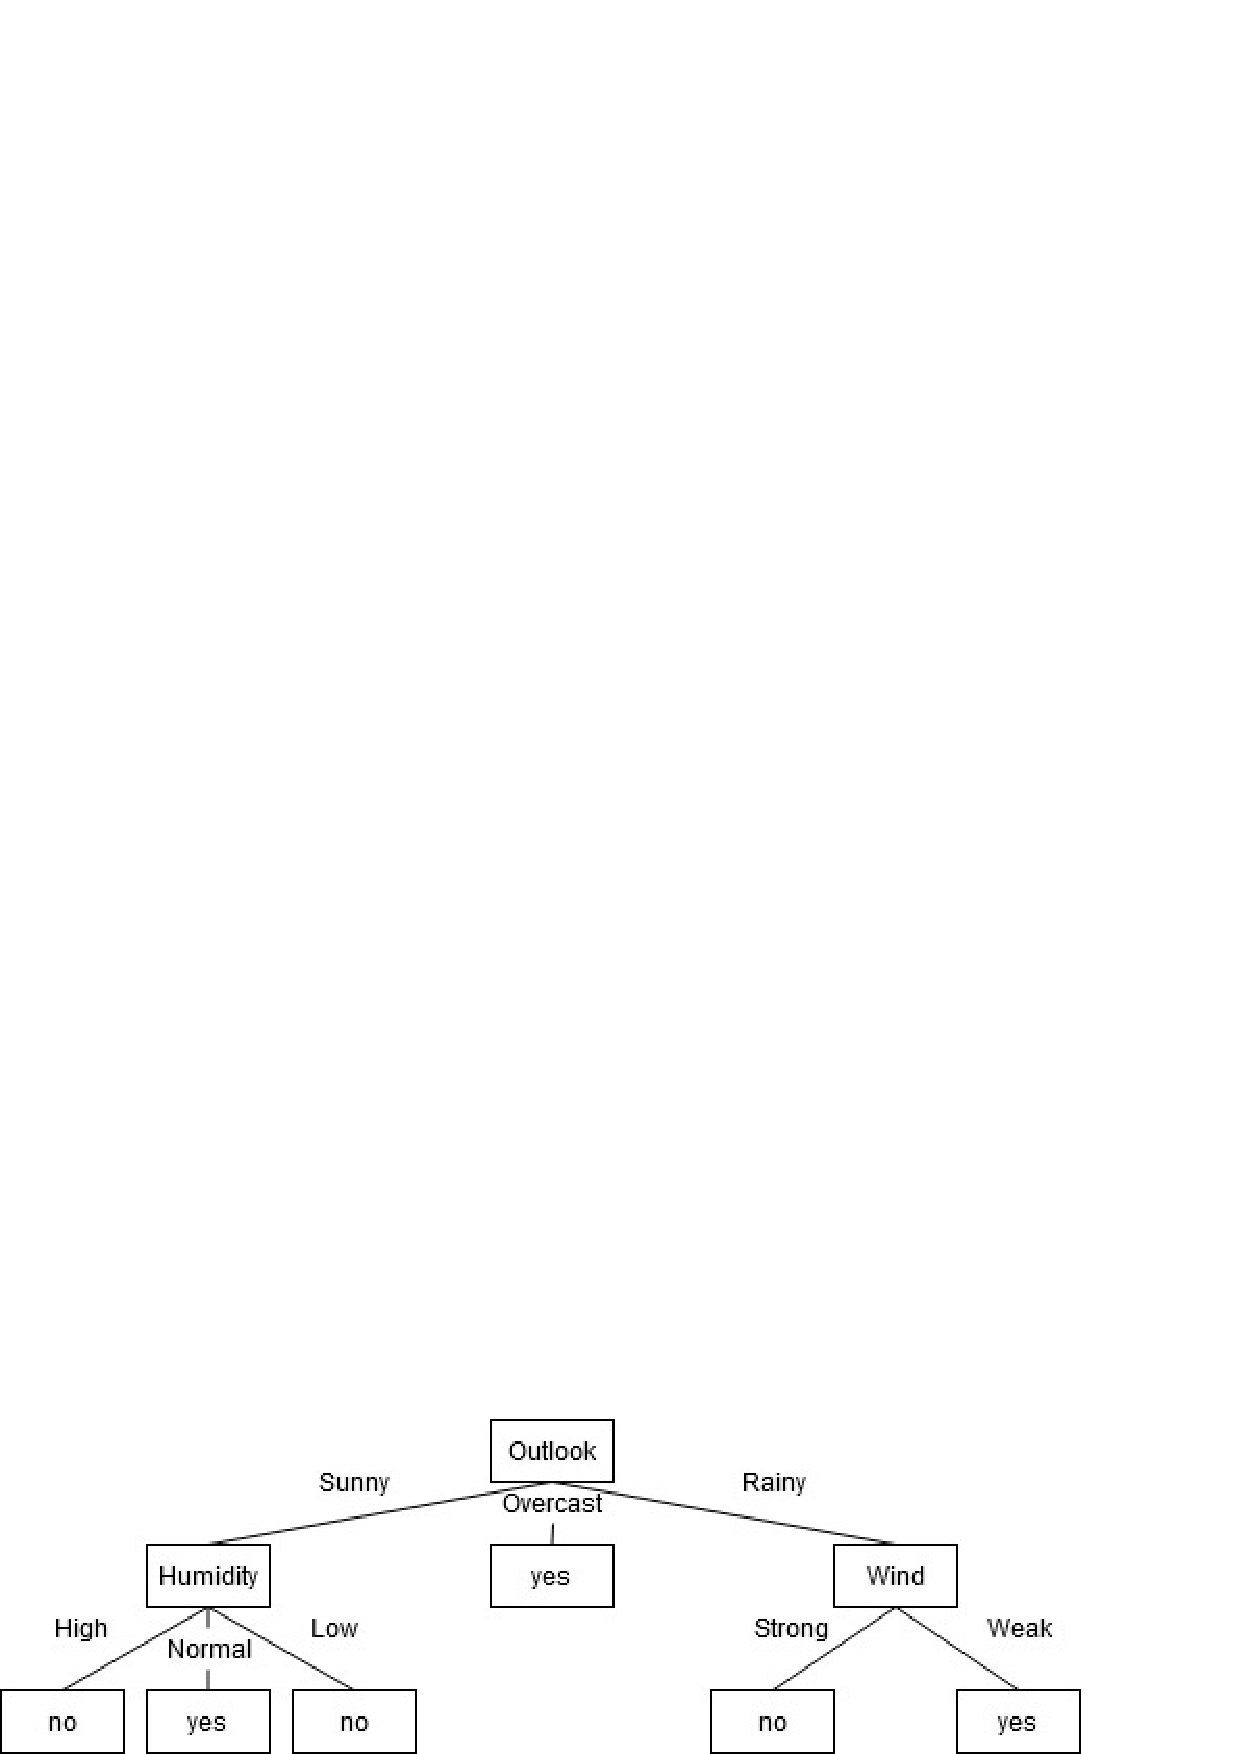
\includegraphics{cs5350hw1_2a.jpg}
	\item~
	\newline similar to part a above but using the Gini Index to calculate the information gain
	\newline First split:
	\newline -Outlook:
	\newline $S_s = 1, 2,8, 9, 11; p^+=2/5; Gini Index=.48$
	\newline $S_o=3, 7, 12, 13; p^+=4/4 = 1; Gini Index=0$
	\newline $S_r=4, 5, 6, 10, 14; p^+=3/5; Gini Index=.48$
	\newline $Information Gain=.46-\frac{5}{14}\cdot(.48+.48)=.12$
	\newline -Temperature:
	\newline $S_h = 1, 2, 3, 13; p^+=1/2; Gini Indexr=.5$
	\newline $S_m=4, 8, 10, 11, 12, 14; p^+=2/3; Gini Index=.44$
	\newline $S_c=5, 6, 7, 9; p^+=3/4; Gini Index=.38$
	\newline $Information Gain=.46-\frac{4\cdot.5+6\cdot.44+4\cdot.38}{14}=.02$
	\newline -Humidity:
	\newline $S_h = 1, 2, 3, 4, 8, 12, 14; p^+=3/7; Gini Index=.49$
	\newline $S_n=5, 6, 7, 9, 10, 11, 13; p^+=6/7; Gini Index=.24$
	\newline $S_l=none$
	\newline $Information Gain=.46\cdot\frac{7\cdot.49+7\cdot.24}{14} = .09$
	\newline -Wind:
	\newline $S_s = 2, 6, 7, 11, 12, 14; p^+=1/2; Gini Index=.5$
	\newline $S_w=1, 3, 4, 5, 8, 9, 10, 13; p^+=3/4;Gini Index=.38$
	\newline $Information Gain=.46\cdot\frac{6\cdot.5+8\cdot.38}{14} = .03$
	\newline Outlook has the highest information gain so it will be used to split
	\newline
	\newline Second split of subsets:
	\newline Sunny subset 1, 2, 8, 9, 11:
	\newline -Temperature:
	\newline $S_h = 1, 2; p^+=0; Gini Index=0$
	\newline $S_m=8, 11, 14; p^+=1/2; Gini Index=.5$
	\newline $S_c=9; p^+=1; Gini Index=0$
	\newline $Information Gain=.48-\frac{2}{5}\cdot.5=.28$
	\newline -Humidity
	\newline $S_h = 1, 2, 8; p^+=0; Gini Index=0$
	\newline $S_n=9, 11; p^+=1; Gini Index=0$
	\newline $S_l=none$
	\newline $Information Gain=.48$
	\newline -Wind:
	\newline $S_s = 2,11; p^+=1/2; Gini Index=.5$
	\newline $S_w=1, 8, 9; p^+=1/3; Gini Index=.44$
	\newline $Information Gain=.48-\frac{2}{5}\cdot.5-\frac{3}{5}\cdot.44=.02$
	\newline Humidity has the largest information gain so it is used for the second split of the sunny subset of outlook
	\newline
	\newline The Humidity split has only two possible outcomes: 
	\newline $S_{sh}=1, 2, 8; p^+ =0$
	\newline $S_{sn}=9, 11; p^+ =1$
	\newline so this cannot be split anymore
	\newline
	\newline Overcast subset 3, 7, 12, 13:
	\newline For the overcast subset 3, 7, 12, 13; $p^+=1$ with Gini Index = 0, so this subset always results in 'yes'
	\newline
	\newline Rainy Subset 4, 5, 6, 10, 14:
	\newline -Temperature:
	\newline $S_h = none$
	\newline $S_m=4, 10, 14; p^+=2/3; Gini Index=.44$
	\newline $S_c=5, 6; p^+=1/2; Gini Index=.5$
	\newline $Information Gain=.48-.6\cdot.44-.4\cdot.5=.16$
	\newline -Humidity
	\newline $S_h = 4, 14; p^+=1/2; Gini Index=.5$
	\newline $S_n=5, 6, 10; p^+=2/3; Gini Index=.44$
	\newline $S_l=none$
	\newline $Information Gain=.48-.4\cdot.5-.6\cdot.44=.16$
	\newline -Wind:
	\newline $S_s = 6, 14; p^+=0; Gini Index=0$
	\newline $S_w=4, 5, 10; p^+=1;Gini Index=0$
	\newline $Information Gain=.48$
	\newline Wind has the largest information gain from the rainy subset so it will be chosen to split. 
	\newline
	\newline The split subsets from the Rainy subset are:
	\newline $S_{rs}=6, 14; p^+=0; Gini Index = 0$
	\newline $S_{rw}=4, 5, 10; p^+=1; Gini Index = 0$
	\newline So the final result can be determined from this subset
	\newline
	\newline Final tree using Gini Index (Result is the same as part a):
	\newline
	\newline 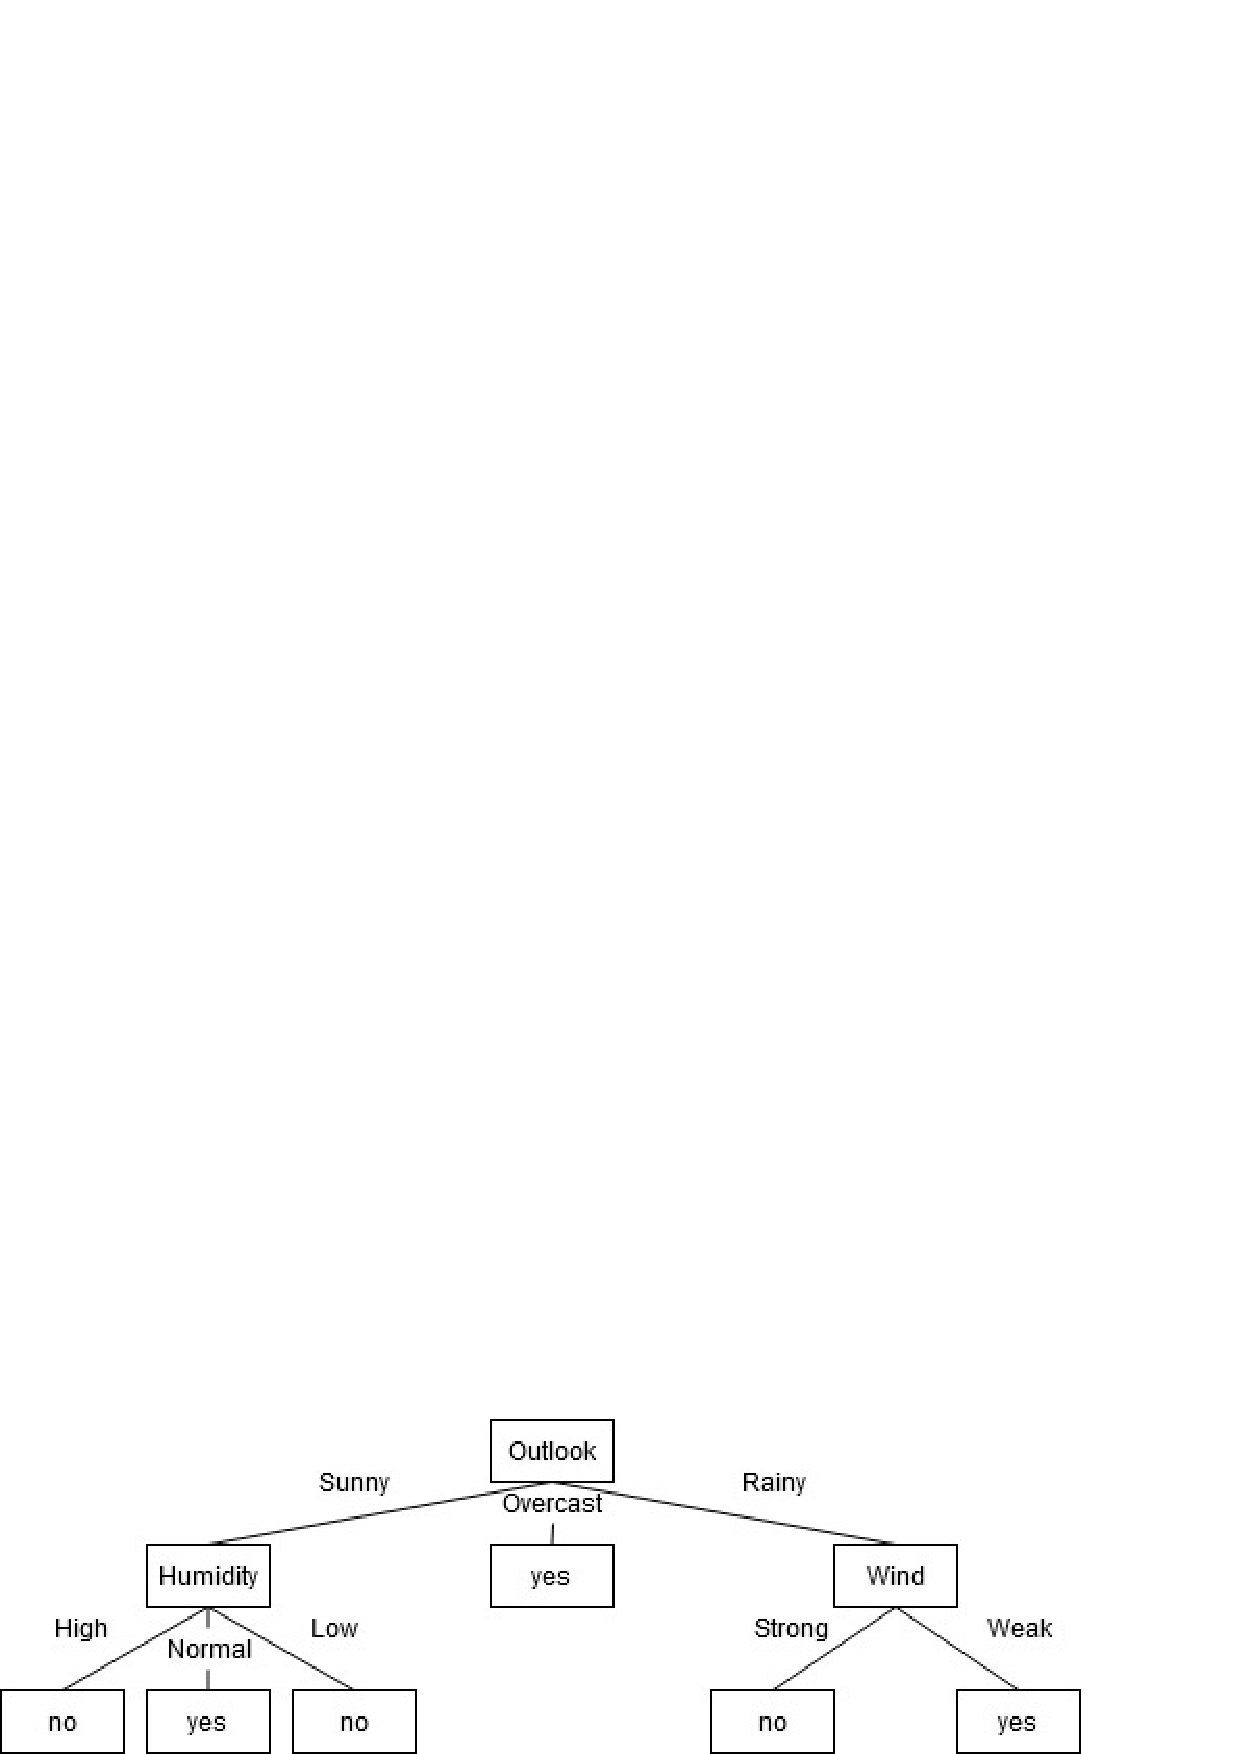
\includegraphics{cs5350hw1_2a.jpg}
	\item~
	\newline The trees from parts a and b are the same as the tree discussed in lecture. This is beacuse the algorithm always results in the same tree structure even if the information gain is calculated differently. Both the Majority Error and Gini Index functions work for this algorithm so the result should be the same. 
\end{enumerate}

\item~ 
\begin{enumerate}
\item~
\newline -Outlook:
	\newline $S_s = 1, 2,8, 9, 11, 15; p^+=1/2; gain=1$
	\newline $S_o=3, 7, 12, 13; p^+ = 1;  gain=0$
	\newline $S_r=4, 5, 6, 10, 14; p^+=3/5;  gain=.97$
	\newline $Information Gain=.92-\frac{6\cdot1+4\cdot0+5\cdot.97}{15}=.197$
	\newline -Temperature:
	\newline $S_h = 1, 2, 3, 13; p^+=1/2; gain=1$
	\newline $S_m=4, 8, 10, 11, 12, 14, 15; p^+=5/7; gain=.86$
	\newline $S_c=5, 6, 7, 9; p^+=3/4;  gain=.81$
	\newline $Information Gain=.92-\frac{4+7\cdot.86+4\cdot.81}{15}=.04$
	\newline -Humidity:
	\newline $S_h = 1, 2, 3, 4, 8, 12, 14; p^+=3/7;  gain=.99$
	\newline $S_n=5, 6, 7, 9, 10, 11, 13, 15; p^+=7/8;  gain=.54$
	\newline $S_l=none$
	\newline $Information Gain=.92-\frac{7\cdot.99+8\cdot.54}{14}=.17$
	\newline -Wind:
	\newline $S_s = 2, 6, 7, 11, 12, 14; p^+=1/2;  gain=1$
	\newline $S_w=1, 3, 4, 5, 8, 9, 10, 13, 15; p^+=7/9; gain=.76$
	\newline $Information Gain=.92-\frac{6\cdot1+9\cdot.76}{15}=.06$
	\newline
	\newline Outlook has the highest information gain, so it should be the chosen feature to split on. 
\item~
\newline -Outlook:
	\newline $S_s = 1, 2,8, 9, 11; p^+=.4;  gain=.97$
	\newline $S_o=3, 7, 12, 13, 15; p^+ = 1;  gain=0$
	\newline $S_r=4, 5, 6, 10, 14; p^+=3/5;  gain=.97$
	\newline $Information Gain=.92-\frac{5\cdot.97+5\cdot.97}{15}=.27$
	\newline -Temperature:
	\newline $S_h = 1, 2, 3, 13; p^+=1/2;  gain=1$
	\newline $S_m=4, 8, 10, 11, 12, 14, 15; p^+=5/7;  gain=.86$
	\newline $S_c=5, 6, 7, 9; p^+=3/4;  gain=.81$
	\newline $Information Gain=.92-\frac{4+7\cdot.86+4\cdot.81}{15}=.04$
	\newline -Humidity:
	\newline $S_h = 1, 2, 3, 4, 8, 12, 14; p^+=3/7;  gain=.99$
	\newline $S_n=5, 6, 7, 9, 10, 11, 13, 15; p^+=7/8; gain=.54$
	\newline $S_l=none$
	\newline $Information Gain=.92-\frac{7\cdot.99+8\cdot.54}{14}=.17$
	\newline -Wind:
	\newline $S_s = 2, 6, 7, 11, 12, 14; p^+=1/2;  gain=1$
	\newline $S_w=1, 3, 4, 5, 8, 9, 10, 13, 15; p^+=7/9;  gain=.76$
	\newline $Information Gain=.92-\frac{6\cdot1+9\cdot.76}{15}=.06$
	\newline
	\newline Outlook still has the highest information gain, so it should be the chosen feature to split on.
\item~
\newline -Outlook:
	\newline $S_s = 1, 2,8, 9, 11, 15(\frac{5}{15}); p^+=\frac{2+5/14}{5+5/14}=.44; gain=.99$
	\newline $S_o=3, 7, 12, 13, 15(\frac{4}{15}); p^+ = 1; gain=0$
	\newline $S_r=4, 5, 6, 10, 14, 15(\frac{5}{15}); p^+=\frac{3+5/14}{5+5/14}=.63;  gain=.95$
	\newline $Information Gain=.92-\frac{5.36\cdot.99+5.36\cdot95}{15}=.23$
	\newline -Temperature:
	\newline $S_h = 1, 2, 3, 13; p^+=1/2; gain=1$
	\newline $S_m=4, 8, 10, 11, 12, 14, 15; p^+=5/7;  gain=.86$
	\newline $S_c=5, 6, 7, 9; p^+=3/4;  gain=.81$
	\newline $Information Gain=.92-\frac{4+7\cdot.86+4\cdot.81}{15}=.04$
	\newline -Humidity:
	\newline $S_h = 1, 2, 3, 4, 8, 12, 14; p^+=3/7;  gain=.99$
	\newline $S_n=5, 6, 7, 9, 10, 11, 13, 15; p^+=7/8;  gain=.54$
	\newline $S_l=none$
	\newline $Information Gain=.92-\frac{7\cdot.99+8\cdot.54}{14}=.17$
	\newline -Wind:
	\newline $S_s = 2, 6, 7, 11, 12, 14; p^+=1/2;  gain=1$
	\newline $S_w=1, 3, 4, 5, 8, 9, 10, 13, 15; p^+=7/9;  gain=.76$
	\newline $Information Gain=.92-\frac{6\cdot1+9\cdot.76}{15}=.06$
	\newline
	\newline Outlook still has the highest information gain, so it should be the chosen feature to split on.
\item~
\newline Starting from the subsets to continue from part c:
\newline Sunny subset 1, 2, 8, 9, 11, $15(\frac{5}{14})$:
\newline -Temperature:
	\newline $S_h = 1, 2; p^+=0;  gain=0$
	\newline $S_m=8, 11, 15(\frac{5}{14}); p^+=\frac{1+5/14}{2+5/14}=.58;  gain=.98$
	\newline $S_c=9; p^+=1;  gain=0$
	\newline $Information Gain=.99-\frac{2.36\cdot.98}{5.36}$
	\newline -Humidity
	\newline $S_h = 1, 2, 8; p^+=0;  gain=0$
	\newline $S_n=9, 11, 15(\frac{5}{14}); p^+=1; gain=0$
	\newline $S_l=none$
	\newline $Information Gain=.99$
	\newline -Wind:
	\newline $S_s = 2,11; p^+=1/2;  gain=1$
	\newline $S_w=1, 8, 9, 15(\frac{5}{14}); p^+=\frac{1+5/14}{3+5/14}=.4;  gain=.97$
	\newline $Information Gain=.99-\frac{2\cdot1+3.36\cdot.97}{5.36}=.009$
	\newline Humidity has the largest information gain so it is used for the second split of the sunny subset of outlook
	\newline
	\newline The Humidity split has only two possible outcomes: 
	\newline $S_{sh}=1, 2, 8; p^+ =0$
	\newline $S_{sn}=9, 11; p^+ =1$
	\newline so this cannot be split anymore
	\newline
	\newline Overcast subset 3, 7, 12, 13, $15(\frac{4}{15})$:
	\newline For the overcast subset 3, 7, 12, 13, $15(\frac{4}{15})$; $p^+=1$ with  gain = 0, so this subset always results in 'yes'
	\newline
	\newline Rainy Subset 4, 5, 6, 10, 14, $15(\frac{5}{15})$:
	\newline -Temperature:
	\newline $S_h = none$
	\newline $S_m=4, 10, 14, 15(\frac{5}{15}); p^+=\frac{2+5/14}{3+5/14}=.7;  gain=.88$
	\newline $S_c=5, 6; p^+=1/2;  gain=1$
	\newline $Information Gain=.95-\frac{3.36\cdot.88+2}{5.36}=.03$
	\newline -Humidity
	\newline $S_h = 4, 14; p^+=1/2;  gain=1$
	\newline $S_n=5, 6, 10, 15(\frac{5}{14}); p^+=\frac{2+5/14}{3+5/14}=.44;  gain=.88$
	\newline $S_l=none$
	\newline $Information Gain=.95-\frac{2+3.36\cdot.99}{5.36}=.03$
	\newline -Wind:
	\newline $S_s = 6, 14; p^+=0;  gain=0$
	\newline $S_w=4, 5, 10, 15(\frac{5}{14}); p^+=1;  gain=0$
	\newline $Information Gain=.95$
	\newline Wind has the largest information gain from the rainy subset so it will be chosen to split. 
	\newline
	\newline The split subsets from the Rainy subset are:
	\newline $S_{rs}=6, 14; p^+=0;  gain = 0$
	\newline $S_{rw}=4, 5, 10; p^+=1;  gain = 0$
	\newline So the final result can be determined from this subset
	\newline
	\newline Final tree for part d:
	\newline
	\newline 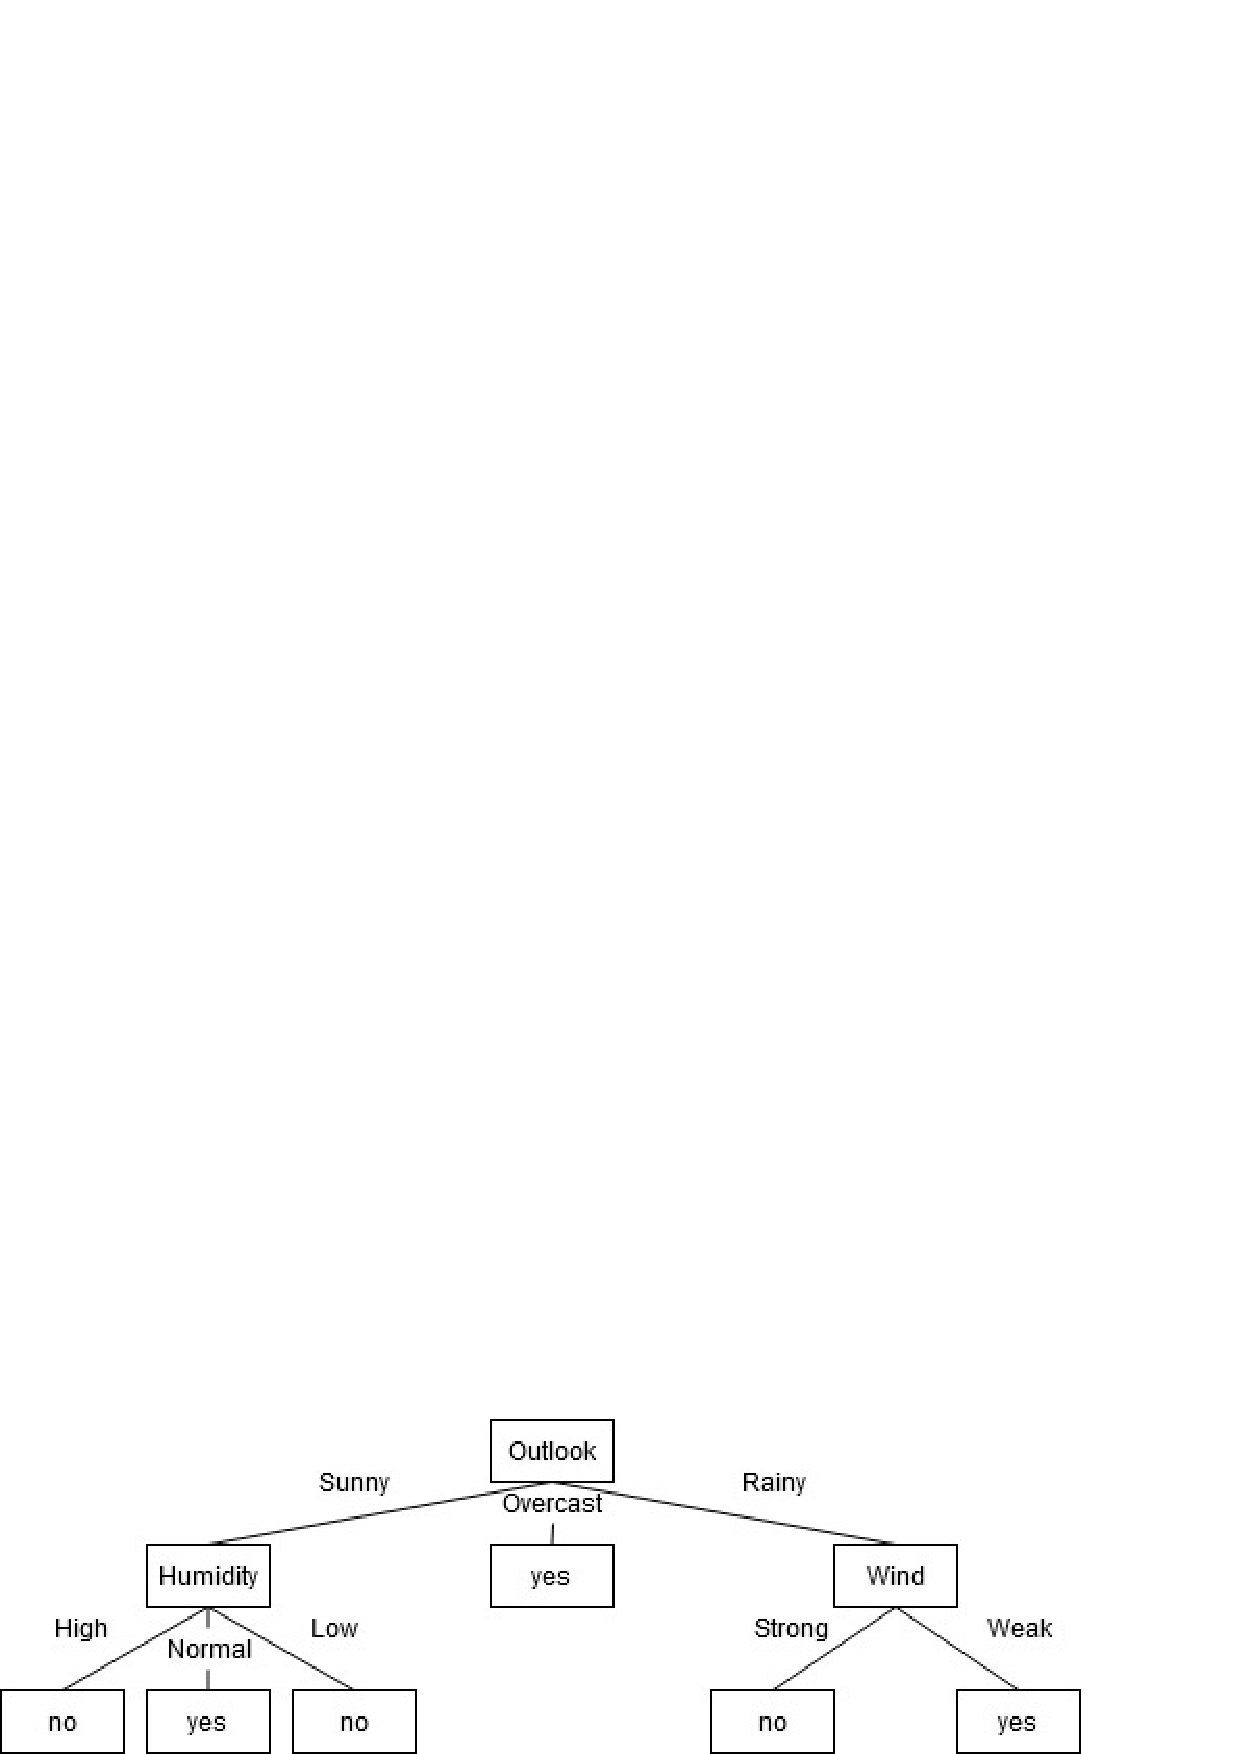
\includegraphics{cs5350hw1_2a.jpg}

\end{enumerate}

\end{enumerate}

\section{Decision Tree Practice}
\begin{enumerate}
	\item~
	\newline GitHub Repository Link: https://github.com/BritGaul/CS5350

\item~
\begin{enumerate}
\item~ 
\newline code for decision tree is in the linked github repository under the DecisionTree directory
\item~
\newline Errors for Training Dataset:
\begin{table}[h]
	\centering
	\begin{tabular}{cccc|c}
		depth & Majority Error & Gini Index & Information Gain\\ 
		\hline\hline
		1 & 30.2 & 30.2 & 30.2 \\ \hline
		2 & 30.01 & 22.2 & 22.2 \\ \hline
		3 & 24.7 & 17.59 & 18.10 \\ \hline
		4 & 21.3 & 8.9 & 8.2 \\ \hline
		5 & 18.01 & 2.7 & 2.7\\ \hline
		6 & 17.20 & 0 & 0\\ \hline
	\end{tabular}
\end{table}

 Errors for Testing Dataset:
\begin{table}[h]
	\centering
	\begin{tabular}{cccc|c}
		depth & Majority Error & Gini Index & Information Gain\\ 
		\hline\hline
		1 & 29.67 & 29.67 & 29.67 \\ \hline
		2 & 31.59 & 22.25 & 22.25\\ \hline
		3 & 26.24 & 18.41 & 19.64 \\ \hline
		4 & 25.96 & 13.74 & 15.11 \\ \hline
		5 & 22.66 & 8.65 & 8.38\\ \hline
		6 & 22.66 & 8.52 & 8.38\\ \hline
	\end{tabular}
\end{table}

\item~
\newline By comparing the training errors and the testing errors, it could be said that using information gain is best approach, because it results in the lowest error for both the training datasets and the testing datasets. The Gini Index errors stay relatively close to the inforamtion gain for both datasets, but the Majoroity Error stays much higher, even when the depth increases.
\newline
\newline
\newline
\newline
\newline
\newline
\newline
\newline
\newline
\newline
\newline
\newline
\newline
\newline
\newline
\end{enumerate}


\item~
\begin{enumerate}
	\item~
	\newline
\newline
\newline
\newline
\newline
\newline
\newline
\newline
\newline
\newline
\newline
\newline
\newline
\newline
\newline
\newline
\newline
\newline
	\newline Errors for Training Dataset:
	\begin{table}[h]
	\centering
	\begin{tabular}{cccc|c}
		depth & Majority Error & Gini Index & Information Gain\\ 
		\hline\hline
		1 & 10.88 & 10.88 & 11.92 \\ \hline
		2 & 10.5 & 10.52 & 10.6 \\ \hline
		3 & 9.76 & 10.1 & 10.22 \\ \hline
		4 & 8.64 & 8.76 & 8.68 \\ \hline
		5 & 7.84 & 7.38 & 7.14\\ \hline
		6 & 7.48 & 5.72 & 5.68\\ \hline
		7 & 7.28 & 4.5 & 4.52 \\ \hline
		8 & 7.20 & 4.5 & 4.52 \\ \hline
		9 & 7.18 & 2.94 & 3.2 \\ \hline
		10 & 7.18 & 2.46 & 2.64 \\ \hline
		11 & 7.18 & 2.24 & 2.34\\ \hline
		12 & 7.18 & 2.20 & 2.22\\ \hline
		13 & 7.18 & 2.20 & 2.22\\ \hline
		14 & 7.18 & 2.20 & 2.22\\ \hline
		15 & 7.18 & 2.20 & 2.22\\ \hline
		16 & 7.18 & 2.20 & 2.22\\ \hline
	\end{tabular}
\end{table}

Errors for Testing Dataset:
 \begin{table}[h]
	\centering
	\begin{tabular}{cccc|c}
		depth & Majority Error & Gini Index & Information Gain\\ 
		\hline\hline
		1 & 12.48 & 11.66 & 12.48  \\ \hline
		2 & 11.02 & 11.53 & 11.26 \\ \hline
		3 & 11.78 & 10.93 & 10.98 \\ \hline
		4 & 11.58 & 11.64 & 11.78 \\ \hline
		5 & 11.60 & 12.26 & 12.74\\ \hline
		6 & 11.96 & 13.26 & 13.64\\ \hline
		7 & 11.96 & 14.30 & 14.32 \\ \hline
		8 & 12.04 & 15.48 & 15.24 \\ \hline
		9 & 12.08 & 16.00 & 16.14 \\ \hline
		10 & 12.14 & 16.24 & 16.88 \\ \hline
		11 & 12.14 & 16.56 & 16.88\\ \hline
		12 & 12.14 & 16.52 & 17.08\\ \hline
		13 & 12.14 & 16.58 & 17.04\\ \hline
		14 & 12.14 & 16.58 & 17.04\\ \hline
		15 & 12.14 & 16.58 & 17.04\\ \hline
		16 & 12.14 & 16.58 & 17.04\\ \hline
	\end{tabular}
\end{table}
	
	
	\item~
	\newline
\newline
\newline
\newline
\newline
\newline
\newline
\newline
\newline
\newline
\newline
\newline
\newline
\newline
\newline
\newline
\newline
\newline
\newline
\newline
\newline
\newline
\newline
\newline
\newline
\newline
\newline
\newline
\newline
\newline
\newline
\newline
\newline
\newline
	\newline Errors for Training Dataset:
	\begin{table}[h]
	\centering
	\begin{tabular}{cccc|c}
		depth & Majority Error & Gini Index & Information Gain\\ 
		\hline\hline
		1 & 10.88 & 10.88 & 11.92 \\ \hline
		2 & 10.5 & 10.52 & 10.6 \\ \hline
		3 & 9.76 & 10.1 & 10.22 \\ \hline
		4 & 8.64 & 8.76 & 8.68 \\ \hline
		5 & 7.84 & 7.38 & 7.14\\ \hline
		6 & 7.48 & 5.72 & 5.68\\ \hline
		7 & 7.28 & 4.5 & 4.52 \\ \hline
		8 & 7.20 & 4.5 & 4.52 \\ \hline
		9 & 7.18 & 2.94 & 3.2 \\ \hline
		10 & 7.18 & 2.46 & 2.64 \\ \hline
		11 & 7.18 & 2.24 & 2.34\\ \hline
		12 & 7.18 & 2.20 & 2.22\\ \hline
		13 & 7.18 & 2.20 & 2.22\\ \hline
		14 & 7.18 & 2.20 & 2.22\\ \hline
		15 & 7.18 & 2.20 & 2.22\\ \hline
		16 & 7.18 & 2.20 & 2.22\\ \hline
	\end{tabular}
\end{table}

Errors for Testing Dataset:
\newline
\newline
\newline
\newline
\newline
\newline
\newline
\newline
\newline
\newline
\newline
\newline
\newline
\newline
\newline
\newline
\newline
\newline
\newline
\newline
\newline
 \begin{table}[h]
	\centering
	\begin{tabular}{cccc|c}
		depth & Majority Error & Gini Index & Information Gain\\ 
		\hline\hline
		1 & 11.60 & 11.66 & 12.48  \\ \hline
		2 & 11.02 & 11.04 & 11.14 \\ \hline
		3 & 11.56 & 10.84 & 10.78 \\ \hline
		4 & 11.58 & 11.64 & 11.78 \\ \hline
		5 & 11.60 & 12.26 & 12.74\\ \hline
		6 & 11.96 & 13.26 & 13.64\\ \hline
		7 & 11.96 & 14.30 & 14.32 \\ \hline
		8 & 12.04 & 15.48 & 15.24 \\ \hline
		9 & 12.08 & 16.00 & 16.14 \\ \hline
		10 & 12.08 & 16.24 & 16.88 \\ \hline
		11 & 12.08 & 16.56 & 16.88\\ \hline
		12 & 12.08 & 16.52 & 17.08\\ \hline
		13 & 12.08 & 16.54 & 17.06\\ \hline
		14 & 12.08 & 16.54 & 17.06\\ \hline
		15 & 12.08 & 16.54 & 17.06\\ \hline
		16 & 12.08 & 16.54 & 17.06\\ \hline
	\end{tabular}
\end{table}	
	\item~
	\newline The training dataset errors become smaller as the depth of the tree is increased. But for the testing dataset the error goes down as the depth of the tree grows. The training error is always usually smaller then the test error. The error also dropped slightly when unknown was added as a new attribute. 
\end{enumerate}
\end{enumerate}




\end{document}
%%% Local Variables:
%%% mode: latex
%%% TeX-master: t
%%% End:
